\newpage
\section{Redes Neuronales}

\noindent Las redes neuronales artificiales, son modelos predictivos basados en el funcionamiento de las propias neuronas del cerebro. Éstas reciben señales de entrada de las neuronas con las cuales están conectadas, las procesan y envían el resultado a las  neuronas siguientes. 

\noindent La ventaja de este tipo de algoritmos es que en esencia, son un conjunto de parámetros y funciones de activación que pueden ser ajustados para cualquier tarea y cualquier tipo de función a aproximar. Solo hace falta la complejidad del modelo adecuada según Hornik, Stinchcombe y  White \cite{Hornik 1989}.  

\noindent Una neurona artificial es mucho más simple que una neurona. López,  Balsa-Canto y  Oñate, definen una neurona en términos matemáticos \cite{Roberto 2008}. Antes hay que definir los siguientes conceptos, para los cuales se han utilizado como base \cite{Grossi 2007, Neural Designer}.

\noindent Sea un vector aleatorio $\mathbf{x}$ de longitud $p$, llamamos datos de entrada al vector $\mathbf{x}_0$ que representa cada una de las observaciones de las $p$  variables medidas. Por otro lado, se llamará datos de salida al vector $\mathbf{y}_0$ obtenido tras haber introducido en la red neuronal el vector $\mathbf{x}_0$.

\noindent Ahora se detallan todos los elementos de una neurona. 

\begin{defi}
Llamaremos pesos sinápticos $\omega$ de una neurona al vector de $p$ constantes que regulan la importancia de cada entrada en la neurona.  A este vector de pesos sinápticos se le puede añadir un término independiente que únicamente se sumará. Se llama sesgo y se denota como $b$.
\end{defi}

\begin{defi}
Se llama función de activación, $f$ de una neurona artificial a la función que transforma la suma ponderada de las entradas para obtener la salida. 

\noindent Las funciones de activación más habituales son: la función identidad (en este caso, es como si se hiciera una simple suma ponderada de los datos de entrada) , la función sigmoide, la tangente hiperbólica o la función lineal rectificada para casos de regresión, es decir, en casos en los que la variable respuesta sea continua. En caso contrario, se pueden utilizar la función softmax o la función logística, ya que devuelven valores en el intervalo $[0,1]$ y se puede asociar con la probabilidad de pertenecer a una clase u otra. 
\end{defi}

\begin{defi}
Una neurona artificial procesa una entrada $\textbf{x}$ de acuerdo con unos pesos sinápticos $(b,\omega)$ que luego es transformada por una función de activación $f(\mathbf{x})$.

\noindent Una  vez definidos los elementos que forman una neurona artificial se puede definir la siguiente función:
\begin{equation}
\begin{split}
g:\mathbb{R}^p &\longrightarrow \mathbb{R}\\
g(\textbf{x})&\longrightarrow g(\textbf{x};b,\omega)
\end{split}
\end{equation}
\begin{equation}
g(\textbf{x})=f\left(b+\sum_{i=1}^p \omega_i x_i\right)
\end{equation}
El siguiente diagrama \ref{fig:neurona-biológica} proporciona una forma sencilla de entender el funcionamiento de dicho modelo, incluyendo la analogía de las neuronas biológicas. 
\end{defi}
\begin{figure}
\begin{center}
%%Hay que pedirle a Carlos que lo edite por que yo la verdad que no se 
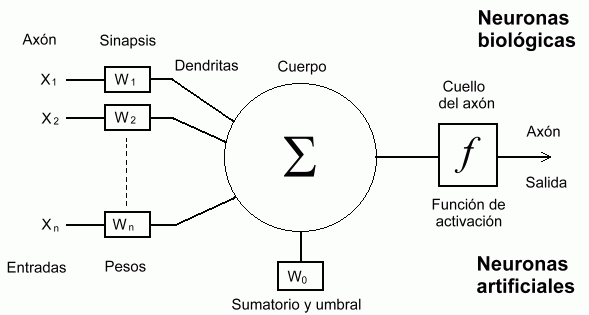
\includegraphics[scale=0.6]{Documentos Extra/Imagenes/neurona.png}
\caption{Representación de una neurona en la que se comparan los elementos biológicos y artificiales. Obtenida de \cite{Requena}}
\label{fig:neurona-biológica}
\end{center}
\end{figure}


\noindent La principal ventaja de estos métodos es que las neuronas se pueden conectar entre ellas, es decir, estas se pueden organizar de manera que los datos de salida de un conjunto de neuronas sirvan como  entrada del siguiente.

\begin{defi}
Se llama capa de neuronas al conjunto de neuronas artificiales que tienen el mismo conjunto de datos de entrada y cuyos datos de salida son la entrada del siguiente.
\end{defi}
\noindent Se pueden establecer varios tipos de capas de neuronas \cite{Neural Designer}:
\begin{defi}
Se llama capa de entrada a la primera capa de neuronas que recibe los valores de las observaciones y las estandariza (Se debe entrenar al modelo para ello).
\end{defi}
\begin{defi}
Se llama capa oculta a cada una de las capas intermedias que se utilizan en las redes neuronales. 
\end{defi}

\begin{defi}
Se llama capa de salida a la última capa que tiene tantas neuronas como variables respuesta y sus datos de salida son las predicciones que hace la red neuronal de las variables respuesta. 
\end{defi}

\noindent Para el proceso de ajuste se utiliza de manera habitual el método del gradiente con un conjunto de datos con $N$ observaciones. En el capitulo  11 Hastie et.al.  detallan en profundidad el ajuste \cite{Hastie 2001}. A este proceso se le llama \emph{back-propagation}, ya que una vez aplicado el método del gradiente se van actualizando los parámetros anteriores. 

\noindent Si queremos expresar el modelo de manera concisa, la complejidad de interpretación aumenta significativamente al expandir la red neuronal. Incluso en casos simples como en la figura  \ref{fig:estructura red neuronal} la interpretación se vuelve complicada. Por lo tanto, las redes neuronales se utilizan principalmente con propósitos predictivos, en lugar de brindar una explicación clara de los parámetros y relaciones involucrados en el modelo \cite{Hastie 2001, James 2013}.

\noindent Las principales ventajas de las redes neuronales es que pueden ajustarse a cualquier estructura sin conocerla a priori. Por otro lado, debido a la gran cantidad de parámetros a ajustar pueden tender al sobreajuste.

\noindent La siguiente imagen \ref{fig:estructura red neuronal} es una representación de una red neuronal como un grafo, en el que cada nodo es una neurona, en particular, los capas azules son capas ocultas, formando cinco capas ocultas, mientras que las amarillas son capas de entrada, y las rojas de salida. 

\begin{figure}[ht]
\centering
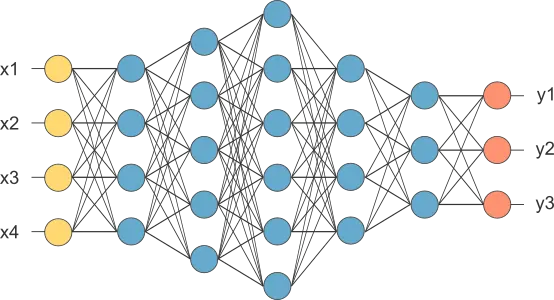
\includegraphics[scale=0.35]{Documentos Extra/Imagenes/red-neuronal-grande.png}
\caption{Imagen extraída directamente de www.neuraldesigner.com}
\label{fig:estructura red neuronal}
\end{figure}


\noindent En esta memoria se han detallado los tipos más básicos de neuronas. Hay tareas específicas que este tipo de neuronas no pueden afrontar, por ejemplo, en el caso de datos que proceden de series temporales en las que estados previos influyen en los estados futuros como puede ser predicciones meteorológicas, bursátiles y otros. Es por ello que  se han desarrollado un tipo más complejo de neuronas llamadas LSTM \emph{(Long-Short Term Memory)} de las que se puede ver su desarrollo y definición además de las propiedades que poseen en \cite{Hochreiter 1997,Neural Designer}.

